\hypertarget{Cheddar_8cpp}{}\section{Cheddar.\+cpp File Reference}
\label{Cheddar_8cpp}\index{Cheddar.\+cpp@{Cheddar.\+cpp}}


\hyperlink{classCheddar}{Cheddar} AI for battleships.  


{\ttfamily \#include $<$iostream$>$}\\*
{\ttfamily \#include $<$cstdio$>$}\\*
{\ttfamily \#include \char`\"{}Cheddar.\+h\char`\"{}}\\*
Include dependency graph for Cheddar.\+cpp\+:\nopagebreak
\begin{figure}[H]
\begin{center}
\leavevmode
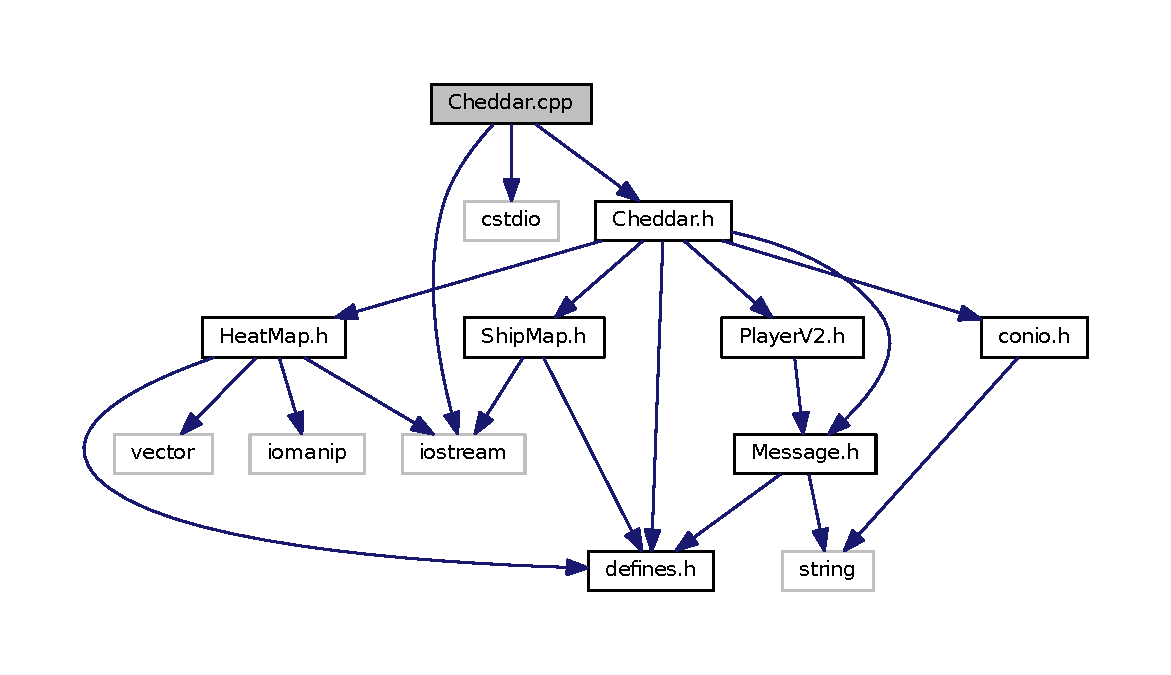
\includegraphics[width=350pt]{Cheddar_8cpp__incl}
\end{center}
\end{figure}


\subsection{Detailed Description}
\hyperlink{classCheddar}{Cheddar} AI for battleships. 

\begin{DoxyAuthor}{Author}
Stefan Brandle, Jonathan Geisler, Jordan Wood, David Fletcher, Ryan Houck 
\end{DoxyAuthor}
\begin{DoxyDate}{Date}
September, 2004, Updated 2015 for multi-\/round play, last modified April 14, 2018 to make an improved AI
\end{DoxyDate}
This Battleships AI is the 2018 Spring code written by Jordan Wood, David Fletcher, and Ryan Houck (based upon Dr. Brandle and Dr. Geisler\textquotesingle{}s base code that placed ships in the top left corner and shot from left to right, then top to bottom). 